
\section{Evaluation Report Targets Table}
\label{sec:eval_report_targets}

\hl{TODO: describe eval target table}

\subsection{Targets of Interest}
\label{sec:eval_targets_of_interest}

\hl{TODO: update screenshots, check section}

\begin{figure}[H]
  \hspace*{-2cm}
    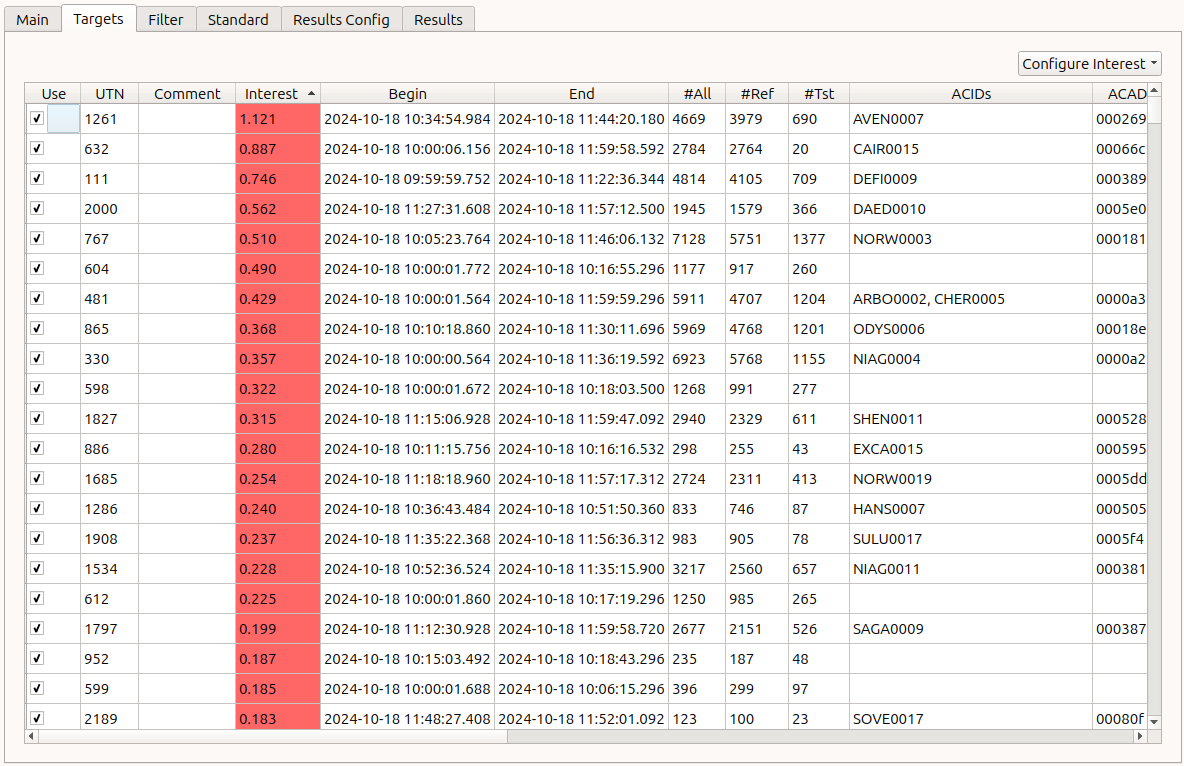
\includegraphics[width=18cm,frame]{figures/eval_targets_eval.png}
  \caption{Evaluation Targets tab with evaluated data}
\end{figure}

After running an evaluation, in the Evaluation Targets tab, the displayed interest is a numerical score showing how strong a negative impact a target had on all requirement results. \\

The interest factor is calculated by:
\begin{itemize}  
\item Stepping through all targets in all given sectors and requirements
\item For each target and requirement, the negative contribution of said target to the respective requirement is calculated
\begin{itemize}  
\item Resulting in a value between 0 (no negative impact) and 1 (all negative contributions come from this single target
\end{itemize}
\item For each target an accumulated sum of per-requirement interest factors is calculated
\end{itemize}
\ \\

The coloring is performed as follows:
\begin{itemize}  
\item higher than 0.1: red
\item higher than 0.05 and lower than 0.1: orange
\item 0.05 and below: green
\end{itemize}
\ \\

When right-clicking a target, several options are shown:
\begin{itemize}  
\item Show full UTN: Load all data from the respective target (not just used reference / test data)
\item Show Surrounding Data: Load all data surrounding the target in position and time (e.g. to find association issues)
\item Jump to requirement: Jump to the respective requirement results section
\end{itemize}
\ \\

Using the 'Configure Interest' button, a list of all requirements is given to select which interest values should be aggregated.
\begin{figure}[H]
  \hspace*{-2.5cm}
    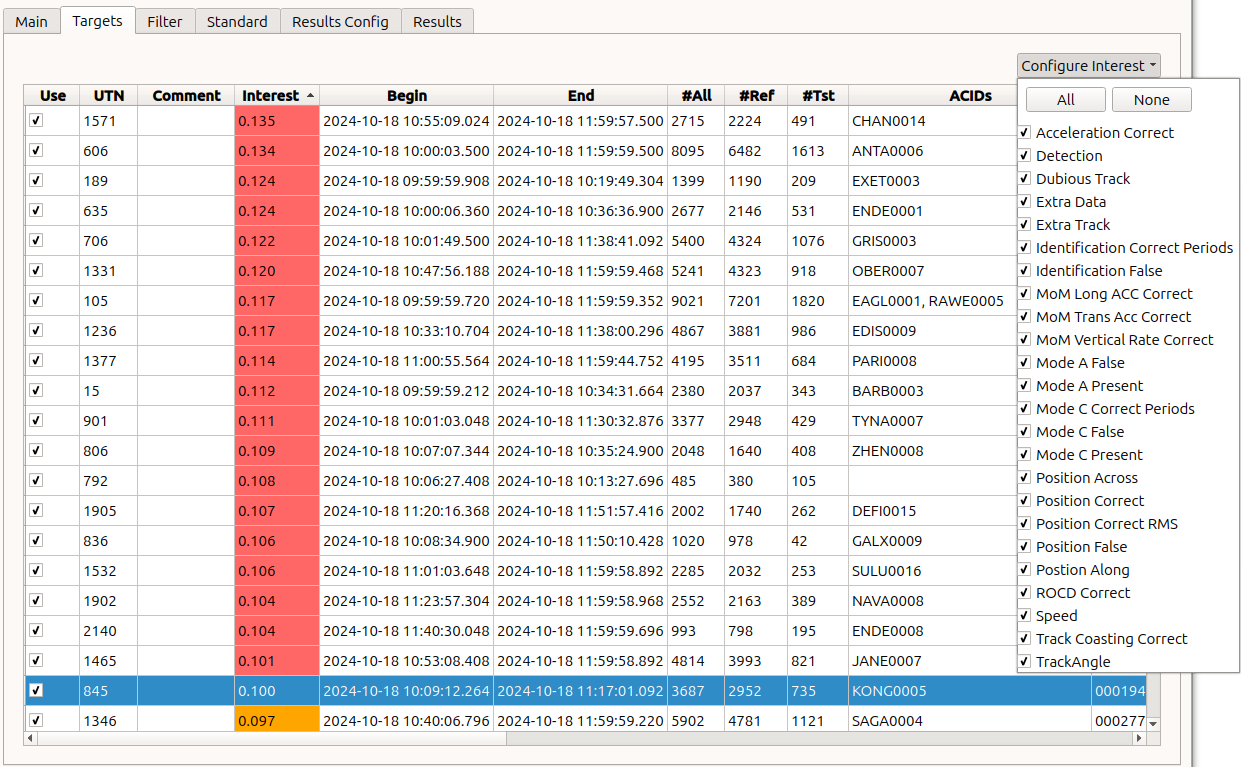
\includegraphics[width=19cm,frame]{figures/eval_targets_config_interest.png}
  \caption{Evaluation Targets: Configure Interest}
\end{figure}
